\documentclass[compress, notes=hide]{beamer}
%\documentclass[compress, notes=hide,handout]{beamer}

\usepackage[english,norsk]{babel} %norske navn rundt omkring
\usepackage{lmodern}
\usepackage[T1]{fontenc} %Norsk tegnsetting (���)
\usepackage[latin1]{inputenc} %Norsk tegnsetting
\usepackage{amsmath,amsfonts,amssymb,mathrsfs} %matematikksymboler
\usepackage{algorithm, algorithmic}
\usepackage{amsthm} %for � lage teoremer og lignende.
\usepackage{bm} %fikser bold math-problematikken
%\usepackage[hang]{subfigure} %hvis du vil kunne ha flere figurer inni en figur
%\usepackage[small,bf,hang]{caption} %bestemmer format p� figurtekst
\usepackage{multirow}
\usepackage{graphpap}
\usepackage{pgf} %Tegning
\def\pgfex{ex}
%\usepackage{mathptmx}
%\usepackage{helvet}
%\usepackage{verbatim}

\setbeamertemplate{caption}[]
\setbeamertemplate{navigation symbols}{}
%\setbeamertemplate{footline}[page number]
\setbeamertemplate{footline}[frame number]
%\setbeamertemplate{caption}[numbered] 
\usecolortheme{default}
%\usetheme{Pittsburgh} %\usetheme{Singapore}
\setbeamertemplate{itemize item}[circle] %triangel p� 2-level-itemize (for 1-level brukt {itemize item})
\setbeamertemplate{itemize subitem}[triangle] %triangel p� 2-level-itemize (for 1-level brukt {itemize item})
\setbeamertemplate{section in toc}[circle]{} %Nummer i table of content
\setbeamertemplate{enumerate items}[circle] 
\setbeamertemplate{itemize subitem}[triangle] %triangel p� 2-level-itemize (for 1-level brukt {itemize item})
\setbeamercolor{itemize subitem}{fg=gray} %farge bullets

% For � skrive i default bl� farge:
% \textcolor[rgb]{0.2,0.2,0.7}{Blablabla-tekst}
%\newcommand{\hl}[1]{\textcolor[rgb]{0.2,0.2,0.7}{\emph{#1}}}
\newcommand{\hl}[1]{\textbf{#1}}
\newcommand{\hlb}[1]{\textcolor[rgb]{0.2,0.2,0.7}{#1}}
\newcommand{\sectionheader}{
    \usebeamerfont*{section number projected}%
    \usebeamercolor{section number projected}%
    \begin{pgfpicture}{-1ex}{-0.4ex}{1ex}{2ex}
      \color{bg}
      \pgfpathcircle{\pgfpoint{0pt}{.75ex}}{1.2ex}
      \pgfusepath{fill}
      \pgftext[base]{\color{fg}\thesection}
    \end{pgfpicture}\kern1.25ex
   \usebeamercolor[bg]{item projected}
    \Large{\insertsectionhead}
}

% FOR Å SKRIVE I DEFAULT, BLÅ FARGE:       \hl{Blablabla-tekst}

\title{Probability and Bayes Law} 
\author{Chi Zhang\\
\footnotesize{Oslo Center for Biostatistics and Epidemiology}\\
\footnotesize{Department of Biostatistics, UiO}\\
\footnotesize{chi.zhang@medisin.uio.no}}
\date{MF9130 -- Introductory Course in Statistics\\
31.01.2023}



\setbeamertemplate{navigation symbols}{}
%\setbeamertemplate{footline}[page number]
\setbeamertemplate{footline}[frame number]
\usecolortheme{default}
%\setbeamertemplate{background}[grid][step=0.25cm]%Rutenett

\begin{document}

\frame{\titlepage}

%DISP:


\section{Overview}

\frame{ 
\frametitle{Outline}
  \begin{block}{Aalen chapter 3.9-3.10, Kirkwood and Sterne chapter 14.4}
    \begin{itemize}
    \item Conditional probability
    \item Law of total probability
    \item Bayes law
    \item Intro to Bayesian statistics
    \end{itemize}
  \end{block}
}

\section{Conditional probability}

% ------ revision of conditional prob 5 min
\frame{ 
\frametitle{Conditional probability}
  \begin{block}{Repetition of conditional probability...}
    \begin{itemize}
    \item The \hl{conditional probability} of $B$ given that $A$ has
      occurred is written
\begin{equation} 
P(B|A) = \frac{P(A \text{ and } B)}{P(A)} \nonumber
\end{equation}
\item \hl{For example}: \vspace{0.5cm}\\
  Probability of a child dying in crib death: ca 1/2000 \\ If a
  sibling has previously died in crib death: about 6/2000 \\ The
  latter is a \emph{conditional} probability
    \end{itemize}
  \end{block}
}

\section{Law of total probability}


% ------ total prob 10 min, one example 

\frame{
\frametitle{Law of total probability}
\begin{block}{Example: Gender of twins}
    \begin{itemize}
    \item We want to find the \hl{probability of two twins having the same gender}
    \item \hl{Monozygotic} twins have the same gender, while \hl{dizygotic} twins
      are like any other siblings
    \item We have to take into consideration if the twins are monozygotic
      or not $\rightarrow$ use \hl{the law of total probability}
    \end{itemize}
\end{block}
}

\frame{ \frametitle{}
\begin{block}{Some notation...}
 \begin{itemize}
 \item $S$ is the \hl{set} of all events
 \item The \hl{union} of $A$ and $B$: \\ \hspace{1cm}
   $A \cup B =$ all events that are in $A$
   \hl{or} $B$
 \item The \hl{intersection} of $A$ and
   $B$: \\ \hspace{1cm} $A \cap B =$ all events that are both in $A$
   \hl{and} $B$
   \item The \hl{complement} of $A$: $\bar{A} = $ all events \hl{not in} $A$  
    \end{itemize}
\hspace{0.5cm}
\begin{center}
\begin{figure}
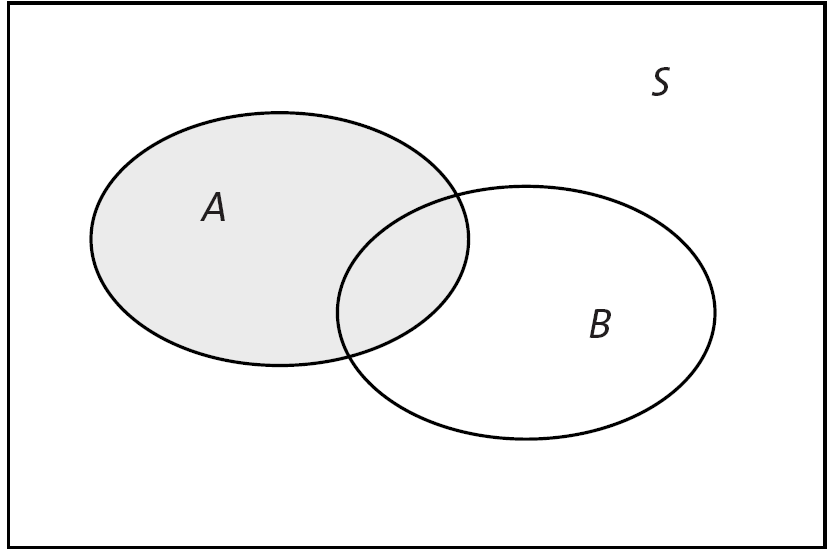
\includegraphics[width=0.45\textwidth]{Figur3-1e.png}
\caption{Venn diagram, where $A = (A \cap B)
  \cup (A \cap \bar{B})$}
\end{figure}
\end{center}
\end{block}
}

\frame{ \frametitle{}
  \begin{center}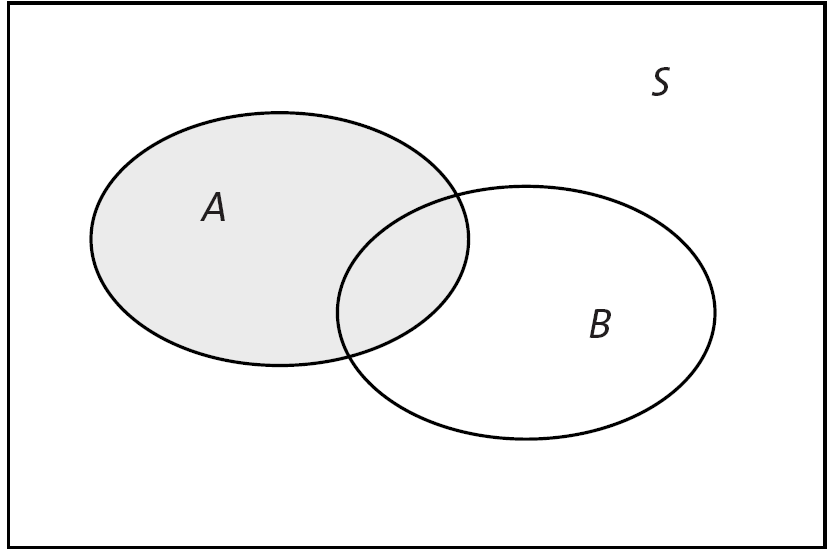
\includegraphics[width=0.35\textwidth]{Figur3-1e.png}\end{center}
\begin{block}{Deriving the law of total probability}
    \begin{itemize}
    \item In the previous slide we saw that \hl{any event A can be
      divided in two} with regard to another event B: \\ $A = (A \cap
      B) \cup (A \cap \bar{B})$
\item Because \hl{the two events are disjunct} we can write: \\
 $P(A) = P(A \cap B) + P(A \cap \bar{B})$
\item Using the multiplicative rule, we get \hl{the law of total
    probability}:\\ \vspace{2mm} $P(A) = P(A|B) P(B) + P(A|\bar{B})
  P(\bar{B})$
    \end{itemize}
\end{block}
}

\frame{
\frametitle{}
\begin{block}{Example: Gender of twins (cont.)}
    \begin{itemize}
    \item A = Both twins have the same gender\\ B = The twins are monozygotic
    \item \hl{Want to find $\bm{P(A)}$}
    \item The probability of twins being monozygotic, $P(B)$, is $1/3$
    \item The law of total probability gives us: \vspace{2mm} \\ $P(A) = P(A|B) P(B) + P(A|\bar{B}) P(\bar{B})$\\\vspace{1mm} \hspace{8.1mm}  $= 1
        \cdot 1/3 + 1/2 \cdot 2/3 $\\ \vspace{1mm} \hspace{8.1mm}  $= 2/3$
     \item The probability that two twins have the same gender is $0.67$
\end{itemize}
\end{block}
}

\section{Bayes law}

% Bayes theorem 15 min

\frame{ 
\frametitle{Bayes law}
\begin{block}{Example: Gender of twins (cont.)}
    \begin{itemize}
    \item What if we now want to find \hl{the probability that two twins
      of the same gender are monozygotic}? 
    \item In other words, what is $P(B|A)$?
    \item \hl{Bayes law} - Thomas Bayes (1702-1761)
    \end{itemize}
\end{block}
\begin{center}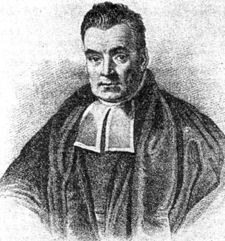
\includegraphics[width=0.18\textwidth]{bayes.png}
\end{center}
}

\frame{ 
\frametitle{}
  \begin{block}{Theory: Bayes law}
    \begin{itemize}    
    \item Remember the definition of
      \hl{conditional probability}, \\
      \vspace{2mm} $P(B|A) = \frac{P(A \cap B)}{P(A)}$,
    \item \hl{the multiplicative rule}, \\ 
      \vspace{2mm} $P(A \cap B) = P(A|B) P(B) = P(B|A) P(A)$, 
    \item and \hl{the law of total probability,}
      $P(A) = P(A|B) P(B) + P(A|\bar{B}) P(\bar{B})$
    \item Combining the three, putting the last two into the first one, gives us the \hl{Bayes law}:\\ \vspace{3mm} $P(B|A)
      = \frac{P(A \cap B)}{P(A)} = \frac{P(A|B) P(B)}{P(A|B) P(B) +
        P(A|\bar{B}) P(\bar{B})}$
      \end{itemize}
   \end{block}
}

\frame{ 
\frametitle{}
\begin{block}{Example: Gender of twins (cont.)}
    \begin{itemize}
    \item Remember:\\ A = Both twins have the same gender\\ B = The twins are monozygotic
      
    \item What is \hl{the probability that two twins of the same gender
      are monozygotic}? In other words, what is $P(B|A)$?
    \item Bayes law gives us:\\
      \vspace{2mm} $P(B|A) = \frac{P(A|B) P(B)}{P(A|B) P(B) +
        P(A|\bar{B}) P(\bar{B})}$\\ \vspace{1mm} \hspace{1.2cm} $=
      \frac{1 \cdot 1/3}{1 \cdot 1/3 + 1/2 \cdot 2/3}$\\ \vspace{2mm}
      \hspace{1.2cm} $ = 1/2$
    \end{itemize}
\end{block}
}




\section{Bayesian statistics}

% intro to bayesian 5-10 min 

\frame{ 
\frametitle{Bayesian statistics}
  \begin{block}{Bayesian statistics: subjective probabilities}
    \begin{itemize}
    \item Although a concept used in everyday live,
      \hl{probability} is difficult to define
      exactly
    \item \hl{Frequentist} definition: the
      probability of an event is the proportion of times that the
      event would occur in a large number of similar trials
    \begin{itemize}
    \item Estimation is completely data driven
    \end{itemize}
  \item \hl{Bayesian} definition: the size of
    the probability represents ones degree of belief in the occurrence
    of an event
    \begin{itemize}
    \item Driven by data AND your prior belief
    \end{itemize}
    \end{itemize}
  \end{block}
}

\frame{ 
\frametitle{}
  \begin{block}{Where does Bayes come in?}
    \begin{itemize}
    \item Bayes law is used to calculate such probabilities based on
      our prior belief: 
      \begin{equation}
        P(\theta|\text{data}) = \frac{P(\text{data}|\theta)P(\theta)}{P(\text{data})} \nonumber
      \end{equation}
    \item $\theta$ refers to the parameters in your model (mean,
      variance, etc.)
    \item The \hl{prior} distribution
      $P(\theta)$ is where you put in your prior beliefs
    \item What you want to estimate is the
      \hl{posterior} distribution
      $P(\theta|\text{data})$, the probability distribution of the
      model parameters given your data
    \item The more data you have, the more will it dominate over your prior belief
    \end{itemize}
  \end{block}
}

\frame{ 
\frametitle{}
  \begin{block}{Bayesian statistics and applications}
    \begin{itemize}
    \item When you have \hl{prior knowledge} about your problem, you get to
      actually use this information
    \begin{itemize}
      \item Was controversial in the beginning, due to the huge change in focus
   \end{itemize}
    \item When you know little (or nothing) of your problem, there are anyway many
      \hl{methodological advantages} in using Bayesian statistics
    \begin{itemize}
    \item Non informative priors: pretend to know very
      little, for ex. prior around 0 with great uncertainty. Then, the
      results are the same as when using frequentist methods
    \item Easier to use than frequentist methods in many advanced problems
   \end{itemize}
    \item Bayesian statistics is not really relevant for simpler
      problems like in this course, but you will (probably) \hl{at some
      point come across papers using Bayesian approaches}
    \end{itemize}
  \end{block}
}

%% \frame{ 
%% \frametitle{}
%%   \begin{block}{Bayesian statistics: Subjectice probabilities}
%%     \begin{itemize}
%%     \item What if the prevalence is unknown? Replace it with a
%%       subjective estimate. Pairs of terms:
%%     \begin{itemize}
%%     \item prevalence $\rightarrow$ apriori probability
%%     \item positive predictive value, negative predictive value
%%       $\rightarrow$ aposteriori probability
%%     \end{itemize}
%%     \item Bayes theorem is used to update probabilites as new
%%       information appear
%%     \item Just as you would update your opinion about something, when
%%       you get new information
%%     \end{itemize}
%%   \end{block}
%% }

%% \frame{ 
%% \frametitle{}
%%   \begin{block}{Example: The lie detector}
%%     \begin{itemize}
%%     \item Is the lie detector reliable?
%%     \item Measures:
%%     \begin{itemize}
%%     \item Respiration
%%     \item  Blood pressure
%%     \item Blood flow
%%     \item Perspiration
%%     \end{itemize}
%%   \item Can bad conscience (guilt) be distinguished from nervousness,
%%     stress etc?
%%     \end{itemize}
%%     \begin{center}
%%       \includegraphics[height=0.3\textheight]{bayes13.png}
%%     \end{center}
%%   \end{block}
%% }




\section{Summary}

\frame{ 
\frametitle{Summary}
  \begin{block}{Key words}
    \begin{itemize}
    \item Conditional probability
    \item Law of total probability
    \item Bayes law
    \end{itemize}
  \end{block}
  \begin{block}{Notation}
    \begin{itemize}
    \item $P(A)$ and $P(\bar{A})$
    \item $P(A|B)$
    \item $P(A\cup B)$ and $P(A\cap B)$
    \end{itemize}
  \end{block}
}


\end{document}

